\begin{frame}
  \frametitle{Results for the Previous Week}

  \begin{center}    
    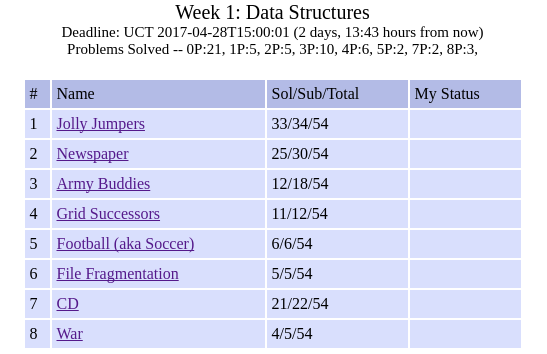
\includegraphics[width=0.45\textwidth]{img/resultsW1_2017}
    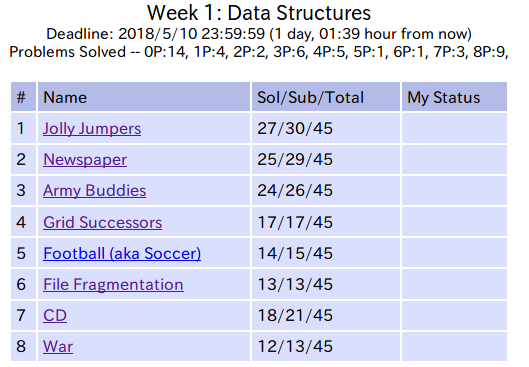
\includegraphics[width=0.45\textwidth]{img/resultsW1_2018}
  \end{center}
\end{frame}

\begin{frame}[fragile]
  \frametitle{Java Speed Hints}

  \begin{itemize}
      \item Don't add strings in a loop:
    {\small
\begin{verbatim}
String a,b;
for (int i = 0; i < N; i++) { a = a + b; } // SLOW!
\end{verbatim}
    }
  \item Use \emph{StringBuilder} instead:
    {\small
\begin{verbatim}
StringBuilder sb; String a,b;
for (int i = 0; i < N; i++) { sb.append(b); }
a = sb.toString();
\end{verbatim}
    }

  \item Java \emph{Arraylist}'s {\bf contain()} is O(n)\footnote{\url{http://stackoverflow.com/questions/10196343/hash-set-and-array-list-performances}}
    {\small
\begin{verbatim}
ArrayList<Int> a;
for (int i = 0; i < N; i++) { a.contain(b); }
\end{verbatim}
    }
  \item Use \emph{HashMap} instead (O(1)):
    {\small
\begin{verbatim}
HashMap<Int> a;
for (int i = 0; i < N; i++) { a.contain(b); }
\end{verbatim}
    }
  \end{itemize}
\end{frame}

\begin{frame}
  \frametitle{Python Speed Hints}
  \begin{block}{Python Speed}
    Some students are also having problems with PYTHON getting
    TLE. (Problem CD).
  \end{block}

  \bigskip
  
  \begin{itemize}
  \item You can still get accepted on CD with python, if you
    remember that the data is \structure{Ordered}!

    \bigskip
    
  \item In general, solutions in python will require better algorithms
    for the bigger problems in this course.
  \end{itemize}
\end{frame}

